
\section{Inference}
\label{section:inference}
In this section, we describe in more detail the inference procedure of the world model and the video decoder.

\subsection{World Model}

\begin{figure}[t]
    \centering 
    \begin{subfigure}{0.32\textwidth}
      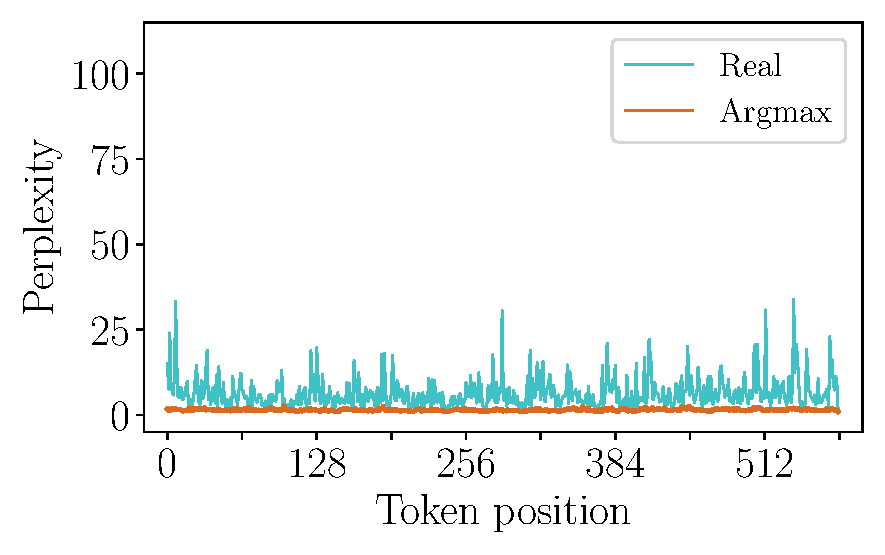
\includegraphics[width=\linewidth]{Figures/Inference/Perplexity/perplexity_argmax.pdf}
      \caption{Argmax.}
    \end{subfigure}\hfill
    \begin{subfigure}{0.32\textwidth}
      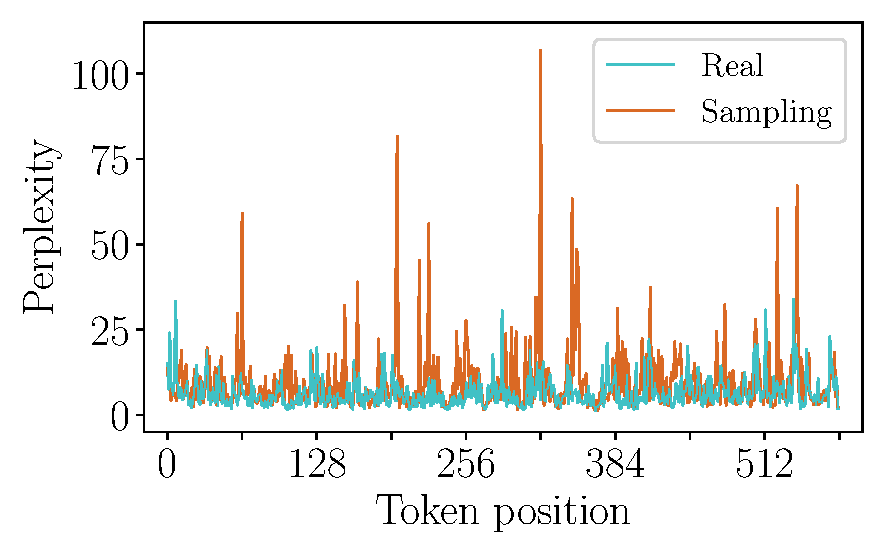
\includegraphics[width=\linewidth]{Figures/Inference/Perplexity/perplexity_sampling.pdf}
      \caption{Sampling.}
    \end{subfigure}\hfill
    \begin{subfigure}{0.32\textwidth}
      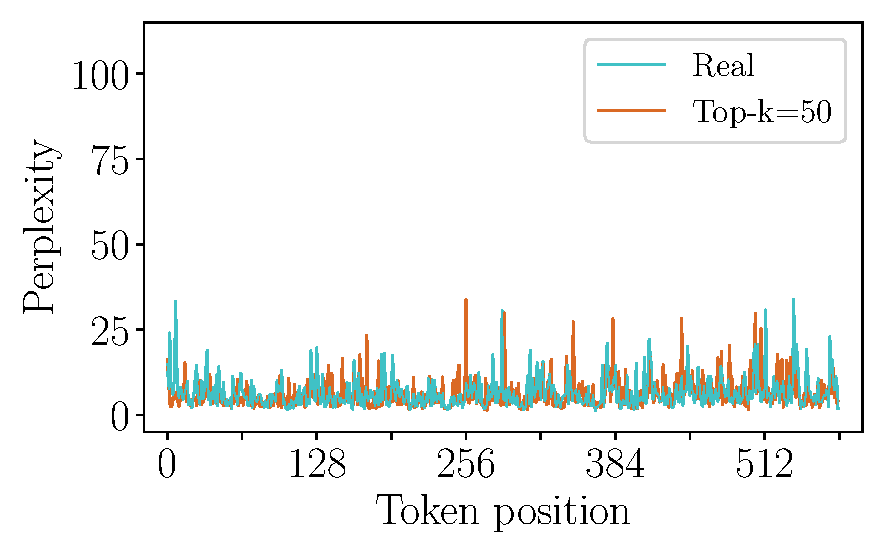
\includegraphics[width=\linewidth]{Figures/Inference/Perplexity/perplexity_topk.pdf}
      \caption{Top-k sampling.}
    \end{subfigure}
\caption{Perplexity of the world model as a function of the position of the generated token. We consider the $n=576$ tokens of a single image frame. We compare the perplexity of the tokens from a real image, to those generated with the following strategies: argmax, sampling, or top-k. In (a), by inspecting the perplexity of a real image we notice it oscillates between low and high values, meaning there is a good range of diversity in those tokens. In contrast, if we look at the argmax strategy, we notice the perplexity only takes extremely low values (no diversity, manifesting in the predicted frames to repeat themselves). Conversely in (b), if we sample from the entire distribution, the perplexity of some tokens can take extremely high values, due to sampling from the unreliable tail. In (c), we observe that top-k=50 sampling produces tokens that have a similar perplexity distribution to real tokens.}
\label{figure:perplexity}
\end{figure}

\paragraph{Sampling.} The world model autoregressively predicts the next image token, conditioned on previous text, image and action tokens. Given the past tokens we perform $n$ forward steps to generate one new image frame. At each step we must sample a token from the predicted logits to select the next token in our sequence. Empirically we observed that maximization-based sampling (i.e. argmax) generates futures that get stuck in a repetitive loop, similarly to language models \citep{holtzman20}. Conversely, if we simply sample from the logits, the selected token can come from the unreliable tail of the probability distribution, which throws the model out-of-distribution, see \Cref{figure:perplexity}.

To encourage diversity as well as realism we employ top-k sampling to sample the next image token from the top-k most likely choices. The chosen value of k is a function of the number of tokens that constitute an image frame as well as the pre-learnt codebook (vocabulary) size.

Our world model can be used to roll out possible futures given starting context as well as generating futures from scratch without any starting context. For long video generation, if the length of the video exceeds the context length of the world model, we employ a sliding window.

\paragraph{Text-conditioning.}The video prediction can be prompted, and thus directed, with text. At training time, we condition our video sequences with text coming from either online narration or offline metadata sources. Because these text sources are imperfect, to improve the alignment between generated futures and the text prompt, we employ classifier-free guidance \citep{ho2022classifier, chang2023muse} at inference time. The effect of guidance is to increase text-image alignment by decreasing the diversity of possible samples. More precisely, for each next token to predict, we compute logits conditioned on text as well as logits with no conditioning (unconditioned). At inference, we can then amplify the differences between the unconditioned and the text-conditioned logits with a scale factor to give the final logits used for sampling.
\begin{equation}
\label{eq:classifier-free-guidance}
l_{\text{final}} = (1 + t)l_{\text{conditioned}} - tl_{\text{unconditioned}}
\end{equation}

By substituting the unconditioned logits with those conditioned on another text prompt, we can perform ``negative'' prompting \citep{negprompt2022}. Pushing the logits away from the negative prompt and towards the positive one encourages the future tokens to include the ``positive'' prompt features while removing the ``negative'' ones.

We found it was important to schedule the scale factor used for guidance over tokens as well as frames. Scheduling over tokens allows some to be sampled with high guidance (hence adhering strongly to the prompt) and others to be sampled with low guidance (hence increasing sample diversity). Scheduling over frames allows for controlling the transition from earlier frames as well as mitigating compounding guidance over subsequent consecutive frames. In \Cref{fig:guidance-schedule} we show an example guidance schedule over twelve frames. Typically we used a schedule that sampled tokens with linearly decreasing guidance over tokens and we lowered the guidance over future frames with a cosine decay, with or without an initial plateau. We note that guidance scale and schedule are hyperparameters to be tuned to particular use cases. 

\begin{figure}[t]
    \centering 
	\begin{subfigure}{0.74\textwidth}
		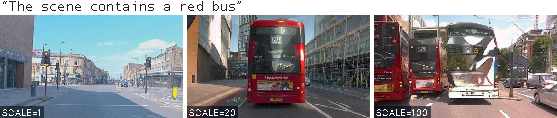
\includegraphics[width=\linewidth]{Figures/Inference/cfg_example.pdf}
		\caption{Guidance scale factor}
	\end{subfigure}\hfil 
	\begin{subfigure}{0.24\textwidth}
		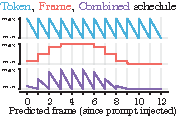
\includegraphics[width=\linewidth]{Figures/Inference/cfg_schedule.pdf}
		\caption{Guidance schedule}
	\end{subfigure}
\caption{Classifier-free guidance.}
\label{fig:guidance-schedule}
\end{figure}




\subsection{Video Decoder}
To decode a sequence of generated tokens from the world model, we use the following video decoding method:

\begin{enumerate}
  \item Decode the first $T'=7$ frames, conditioned on the corresponding $T'$ image tokens.
  \item Autoregressively decode the next $T'-2$ frames, using 2 past overlapping frames as image context, and the following $T'-2$ image tokens.
  \item Repeat the autoregressive process until the $N$ frames have been generated at \SI{6.25}{\hertz}.
  \item Temporally upsample the $N$ frames from \SI{6.25}{\hertz} to \SI{12.5}{\hertz}
  \item Temporally upsample the $2N-1$ frames from \SI{12.5}{\hertz} to \SI{25.0}{\hertz}
\end{enumerate}



We use the DDIM sampler \citep{song2021denoising} with $50$ diffusion steps. During autoregressive decoding, we see a trade-off between reflecting token information content in the generated video and temporal consistency. To balance between these two objectives, we calculate a weighted average of the two tasks \citep{esser2023structure}.
\begin{equation}
\Tilde{\mathbf{\epsilon}}_{\theta}(\rvx^{t'}, t', \rvz, \rvm)
= w\cdot \mathbf{\epsilon}_{\theta}^{\pi}(\rvx^{t'}, t', \rvz, \rvm) + (1-w)\cdot \mathbf{\epsilon}_{\theta}(\mathbf{x}^{t'}, t', \mathbf{z}, \rvm)
\end{equation}

where function $\mathbf{\epsilon}_{\theta}^{\pi}(\rvx^{t'}, t', \rvz, \rvm)$ denoises each frame individually  as images and function $\mathbf{\epsilon}_{\theta}(\mathbf{x}^{t'}, t', \mathbf{z}, \rvm)$ denoises the sequence of frames jointly as a video. In practice, we simply switch on and off the temporal layers. We apply this weighted average randomly for each diffusion step with probability $p=0.25$ and weight $w=0.5$.

While exploring different inference approaches for video decoding we found that decoding video frames autoregressively backwards starting from the end of the sequence led to more stable objects and less flickering on the horizon. In our overall video decoding method, we thus decode the last $T'$ frames and autoregressively decodes the remaining frames backward from there.

%We noticed that decoding video autoregressively-forward from low-resolution tokens results in the model inventing high-frequency details for small objects that we have little information about and leads to temporal inconsistency. To combat this, we decode autoregressively-backwards which makes the generation task easier since we now shrink large objects instead and have additional information about small objects passed through the pixel-space context. In our overall video decoding method, we now generate the last $T'=7$ frames and autoregressively generate the frames backward from there.



